
\newcommand{\rb}[1]{\raisebox{.685cm}{$\; #1 \;$}}


\section{Representation theory}  \label{ss:repthy}

By construction, if the gram matrix of a standard module is singular - i.e. of submaximal rank - then the module map to the corresponding co-standard is of submaximal rank and the standard module has a submodule, and hence there is a morphism in from some other standard module.
By quasiheredity (or globalisation) \cite{KadarYu} the possible maps in are restricted.
In particular in the one-cup cases the possibilities are very restricted, and we 
can identify the module mapping in. 
More generally this identification requires some detective work. 
There is the general {\em tower of recollement} scheme, or we can investigate examples piecemeal. Both approaches are illuminating, and we will work through some cases here. 

\subsection{Generalities}

For each $l$, we can in principle apply the tower of recollement method. 
For $l\geq 0$ 
the tower of recollement method requires an inital `bootstrap' calculation, 
here of morphisms into `1-cup' modules - necessarily from no-cup modules, by globalisation. 
%\ppm{Dump what we have} about the bootstrap here! At least for $l=0$. 

%The case $l=-1$ is classical

\subsubsection{Bootstrap for $l=0$}   \label{ss:bootcase0}

Set $l=0$. 
For definiteness consider $\Delta^{n}_{(n-2,(2))}$ for now, so there is a $(2)$ projector attached to the first two propagating legs of each basis diagram.  


\mdef   \label{exa:l0p6la2-}
Example. 
Explicit  basis for  
$\Deltaa^{l=0,n=6}_{(4,(2))}$ is:  %and ... (not consistent with proper labelling \ppm{yet!}):  
\medskip 

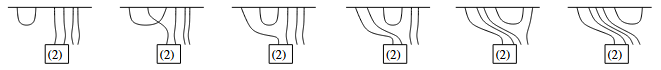
\includegraphics[width=10.9cm]{xfig-ppm/Delta62bas.png}


\mdef  
(We will omit the projector from diagrams for now. And drop the example to $n=5$ for brevity.) 
A 1-d submodule must be spanned by an element of form:
\[ 
\rb{\;a\;} \begin{tikzpicture}[scale=0.68]
     \draw (0,0) -- (2.43,0) ;
     \draw (1.5,0) -- (1.5,-1);
     \draw (1.85,0) -- (1.85,-1);
     \draw (2.2385,0) -- (2.2385,-1);
     \draw (.5,0) .. controls (.5,-.5) and (1.0,-.5) .. (1,0) ;
 \end{tikzpicture}
 \rb{+\;b\;} 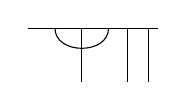
\begin{tikzpicture}[scale=0.68]
     \draw (0,0) -- (2.43,0) ;
     \draw (1,0) -- (1,-1);
     \draw (1.85,0) -- (1.85,-1);
     \draw (2.2385,0) -- (2.2385,-1);
     \draw (.5,0) .. controls (.5,-.5) and (1.5,-.5) .. (1.5,0) ;
 \end{tikzpicture}
\rb{+\;c\;} 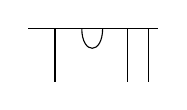
\begin{tikzpicture}[scale=0.68]
     \draw (0,0) -- (2.43,0) ;
     \draw (.5,0) -- (.5,-1);
     \draw (1.85,0) -- (1.85,-1);
     \draw (2.2385,0) -- (2.2385,-1);
     \draw (1.,0) .. controls (1.,-.5) and (1.39,-.5) .. (1.39,0) ;
      \end{tikzpicture}
 \rb{+\;d_1\;} 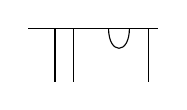
\begin{tikzpicture}[scale=0.68]
     \draw (0,0) -- (2.43,0) ;
     \draw (.5,0) -- (.5,-1);
     \draw (.85,0) -- (.85,-1);
     \draw (2.2385,0) -- (2.2385,-1);
     \draw (1.5,0) .. controls (1.5,-.5) and (1.89,-.5) .. (1.89,0) ;
 \end{tikzpicture}
  \rb{+\; d_2 \;...\;}
\]
(this being a general element of the space with basis as in (\ref{exa:l0p6la2-})).
We are looking for 1d submodules where all algebra defining-basis elements with any cup act as 0. 
Thus for example 
(action of elements with cup and cap in same position, say, taken in the natural order 
- noting that the position of the cup plays no role in determining the coefficients):
\[
\begin{bmatrix}
   x&1& 1 \\ 1&x&1 &1 \\ 1&1&x&1 \\ &1 &1&x&1 \\ &&& 1&x&1 \\ &&&& 1&x&1 \\  &&&&& 1&x&1 \\ &&&&&& 1&x&1 \\ &&&&&&&1&x
\end{bmatrix}
\begin{bmatrix}
    a \\ b \\ c \\ d_1 \\ d_2 \\ \vdots \\ \vdots \\ \vdots
\end{bmatrix}
=0
\]
(other entries 0; we write $x$ for the $\xx$ parameter for now). 
Observe that with this choice the matrix coincides with the gram matrix \cite{ShBr}. 
Evidently we need submaximal rank here, so this coincides, so far, 
with the Chebychev problem we already have (see \S\ref{ss:cheby0}). 
But now let us also require that the first elementary transposition 
$\sigma_1$ acts like +1 (we  consider -1 later, in \ref{case-1}). 

\mdef  
Aside: Observe that all these matrices have manifestly submaximal rank when $x=1$. 
And indeed rank 6 case has another (fairly manifest) linear dependence when $x=1$ (consider row-2 + row-6 vs row-1 + row-5). Is there a pattern? 
%\ppm{[-not quite understanding this case yet! 
(An affine alcove-like effect would manifest as some kind of re-occurrence of special values, such as $x=1$ when $n$ cong. 0 mod. 3.) %???...]} 
Yes.
... Rank 9 has row-1 + row-5 + row-8 = row-2 + row-6 + row-9. 
And the pattern will now be clear. 

%\newcommand{\Deltaaa}[2]{\Deltaa^{#1}_{#2}}

\mdef 
Requiring $\sigma_1$ to act like +1 on our subspace 
(requiring a $\Deltaaa{n}{(n,(2))}$ submodule) %This 
sets $b=c$. 
If $a=0$ then $b+c=0$ so $b=c=0$ and there is no nonzero solution, so here we can take $a=1$. Thus $x+2b=0$ and so $b=c=-x/2$. Thus 
$d_1=-(1-(1+x)x/2) = \frac{x^2 +x-2}{2} =\frac{(x-1)(x+2)}{2}$; then 
$d_2=-(xd_1 +2b) = -x(d_1 -1) =\frac{-x(x^2 +x-4)}{2}$; then 
$d_3=-(xd_2+d_1) = \frac{x^2(x^2+x-4) - (x^2+x-2)}{2} = \frac{x^4 +x^3-5x^2-x+2}{2}$ 
(confer \ref{ss:cheby0})
and so on until $d_{j} = -(xd_{j-1} +d_{j-2})$; 
and finally $xd_{j}=-d_{j-1}$, which is 
$d_{j+1} = -(xd_{j} +d_{j-1})$ provided that $d_{j+1} =0$. 
This last condition gives the $x$ values for which there is a map at each $n$.

\mdef  \label{case-1}
In case $\sigma_1$ acts like -1 
 then also $a=0$ and $b=-c\neq 0$ and $d_i =0$. Thus $xb-b = b-xb=0$ and $x=1$. 
% \ppm{[dont understand this yet!]}
Confer Fig.\ref{fig:Bratelli-l0-gramdets}. 

\mdef For completeness we can consider maps to $\Delta^{n}_{(n-2,(1^2))}$. 
The matrix part is 
\beq \label{eq:l0ev12}
\begin{bmatrix}
   x&1& 1 \\ 1&x&1 &-1 \\ 1&1&x&1 \\ &-1 &1&x&1 \\ &&& 1&x&1 \\ &&&& 1&x&1 \\  &&&&& 1&x&1 \\ &&&&&& 1&x&1 \\ &&&&&&&1&x
\end{bmatrix}
\begin{bmatrix}
    a \\ b \\ c \\ d_1 \\ d_2 \\ \vdots \\ \vdots \\ \vdots
\end{bmatrix}
=0
\eq 
For maps from $(n,(2))$ we require $\sigma_1$ to act as +1. 
Here $b=c$ and $d_i = 0$. 
If $a=0$ then $b+c=0$ from (\ref{eq:l0ev12}) and hence $b=c=0$, so we can assume 
$a=1$ so $x+2b=0$ and $b=-x/2$. 
The second row of  (\ref{eq:l0ev12}) gives 
$1-(x+1)x/2 =d_1 = 0 = -\frac{x^2 +x-2}{2} =-\frac{(x-1)(x+2)}{2}$. 
The rest are automatic. 

Requiring $\sigma_1$ to act as -1 we get $a=0$ and $b=-c$. 
We can put $b=1$.
The second row gives $x-1 = d_1$. The third is automatic. 
The fourth gives $-1-1+x(x-1) =-d_2 = x^2 -x -2 = (x-2)(x+1)$. 
The $d_i$s then satisfy the Chebyshev recurrence until the last step, and we get a solution provided that
$x$ is such that the last $d_i$ is 0.
%... \ppm{[finish me!!]}

\subsubsection{Bootstrap for \ignore{$l=1$ and}general $l$}   \label{ss:keybootl1}
Fix $l$, $\l\vdash l+2$ and $n\geq l+4$. In this subsection we prove that when $\a_0$ is a root of the polynomial $P_{n}^{(\l)}$, the $J_{l,n}(\a_0)$ standard module $\Delta^{n}_{(n-2,\l)}$ has a submodule isomorphic to $\Delta^{n-2}_{(n-2,\l)}$. We proceed as follows.

\ignore{Here the simplest indicative example is for $\Deltaaa{5}{3,(21)}$ given by \ref{exa:keyn5la21}. 
Recall a basis is:
\[
\hspace{-1cm} 
\onecuppppp{6}{1}{2}{3}{4}{5}  \; 
\onecuppppp{6}{1}{3}{2}{4}{5}  \;
\onecuppppp{6}{1}{4}{2}{3}{5}  \;
\onecuppppp{6}{2}{4}{1}{3}{5}  \;
\onecuppppp{6}{2}{3}{1}{4}{5}{}{}  \;
\onecuppppp{6}{3}{4}{1}{2}{5}{}{}  \;
\onecuppppp{6}{4}{5}{1}{2}{3}{}{}  
\]
%
%\medskip 
\[
\hspace{1cm} 
\onecupppppx{6}{1}{2}{3}{4}{5}  \;
\onecupppppx{6}{1}{3}{2}{4}{5}    \;
\onecupppppx{6}{1}{4}{2}{3}{5}  \;
\onecupppppx{6}{2}{4}{1}{3}{5}  \;
\onecupppppx{6}{2}{3}{1}{4}{5}{}{}   \;  
\onecupppppx{6}{3}{4}{1}{2}{5}{}{}  \;
\onecupppppx{6}{4}{5}{1}{2}{3}{}{}  
\]
and so the action of one-cup (one-cap) elements on basis elements is given by, for example: 
\medskip 

%\[   %%%%% begin a diagram 

\hspace{-2.8231cm} 
\flip{\onecupppppo{6}{1}{2}{3}{4}{5}} \hspace{.0031cm}
\flip{\onecupppppo{6}{1}{2}{3}{4}{5}} \hspace{.0041cm}
\flip{\onecupppppo{6}{1}{2}{3}{4}{5}} \hspace{-.004cm}
\flip{\onecupppppo{6}{1}{2}{3}{4}{5}} \hspace{.001cm} 
\flip{\onecupppppo{6}{1}{2}{3}{4}{5}} \hspace{.001cm}
\flip{\onecupppppo{6}{1}{2}{3}{4}{5}} \hspace{.001cm}
\flip{\onecupppppo{6}{1}{2}{3}{4}{5}}

\hspace{-2.791cm} 
\onecuppppp{6}{1}{2}{3}{4}{5}  \; 
\onecuppppp{6}{1}{3}{2}{4}{5}  \;
\onecuppppp{6}{1}{4}{2}{3}{5}  \;
\onecuppppp{6}{2}{4}{1}{3}{5}  \;
\onecuppppp{6}{2}{3}{1}{4}{5}{}{}  \;
\onecuppppp{6}{3}{4}{1}{2}{5}{}{}  \;
\onecuppppp{6}{4}{5}{1}{2}{3}{}{}  

%%%%%%%%%%%%%%%% end a diagram.
\vspace{.321cm}
%%%%%%%  begin a diagram

\hspace{-2.8231cm} 
\flip{\onecupppppo{6}{1}{2}{3}{4}{5}} \hspace{.0031cm}
\flip{\onecupppppo{6}{1}{2}{3}{4}{5}} \hspace{.0041cm}
\flip{\onecupppppo{6}{1}{2}{3}{4}{5}} \hspace{-.004cm}
\flip{\onecupppppo{6}{1}{2}{3}{4}{5}} \hspace{.001cm} 
\flip{\onecupppppo{6}{1}{2}{3}{4}{5}} \hspace{.001cm}
\flip{\onecupppppo{6}{1}{2}{3}{4}{5}} \hspace{.001cm}
\flip{\onecupppppo{6}{1}{2}{3}{4}{5}}

\hspace{-2.81cm} 
\onecupppppx{6}{1}{2}{3}{4}{5}  \;
\onecupppppx{6}{1}{3}{2}{4}{5}    \;
\onecupppppx{6}{1}{4}{2}{3}{5}  \;
\onecupppppx{6}{2}{4}{1}{3}{5}  \;
\onecupppppx{6}{2}{3}{1}{4}{5}{}{}   \;  
\onecupppppx{6}{3}{4}{1}{2}{5}{}{}  \;
\onecupppppx{6}{4}{5}{1}{2}{3}{}{}  

%%%%%%%%%%%% end a diagram.

\medskip 

\noindent 
Observe here that one-cup elements can be written in the form $\uu_{kl} \uu_{ij}^*$; 
and the $\uu_{kl}$ plays essentially no role in the linear algebra of their action, so 
we omit it and our example above has $(i,j)=(1,2)$. 
\\ 
Observe also that 
the remainder of the expression is then encoded as an element of the Specht module 
- provided that we take account of the quotient that is in play. 
Specifically here then, writing $\{ b_1, b_2 ,..., b_{d_\l} \}$ as usual for our Specht module basis (ported into the standard module as per the construction):  
the first term is $\xx b_1$; 
then next is simply $b_1$; 
the next two are both $\sigma_1 b_1 = b_1$ in our chosen basis; 
the next is $b_1$; and 
the next two are zero. 
On the next row: the first is $\xx b_2$; 
the next is $b_2$; 
the next two are $\sigma_1 b_2$ (which can be rewritten as a linear combination); 
the next is $b_2$; and the final two are zero. 
That is, for a general element of the module, with coefficients $\kappa_{hij}$ say for basis elements $\uu_{ij} b_h$, we have  
\[
\uu_{kl} \uu_{12}^* \sum_{hij} \kappa_{hij} \uu_{ij} b_h \; 
        = \; \uu_{kl} ((\xx\kappa_{112} +\kappa_{113}+\kappa_{114} \sigma_1+\kappa_{124}\sigma_1+\kappa_{123}+0+ 0) b_1  + (\xx\kappa_{212} +\kappa_{213}+...+ ...) b_2 ) 
\]
Observe that we can write this as 
\[ ...\]
...

\vspace{.53cm} 

%%%%%%%%%  begin a diagram 

\hspace{-2.8231cm} 
\flip{\onecupppppo{6}{4}{5}{1}{2}{3}} \hspace{.0031cm}
\flip{\onecupppppo{6}{4}{5}{1}{2}{3}} \hspace{.0041cm}
\flip{\onecupppppo{6}{4}{5}{1}{2}{3}} \hspace{-.004cm}
\flip{\onecupppppo{6}{4}{5}{1}{2}{3}} \hspace{.001cm} 
\flip{\onecupppppo{6}{4}{5}{1}{2}{3}} \hspace{.001cm}
\flip{\onecupppppo{6}{4}{5}{1}{2}{3}} \hspace{.001cm}
\flip{\onecupppppo{6}{4}{5}{1}{2}{3}}

\hspace{-2.791cm} 
\onecuppppp{6}{1}{2}{3}{4}{5}  \; 
\onecuppppp{6}{1}{3}{2}{4}{5}  \;
\onecuppppp{6}{1}{4}{2}{3}{5}  \;
\onecuppppp{6}{2}{4}{1}{3}{5}  \;
\onecuppppp{6}{2}{3}{1}{4}{5}{}{}  \;
\onecuppppp{6}{3}{4}{1}{2}{5}{}{}  \;
\onecuppppp{6}{4}{5}{1}{2}{3}{}{}  

%%%%%%%%%%%%%%%% end a diagram.
\vspace{.321cm}
%%%%%%%  begin a diagram

\hspace{-2.8231cm} 
\flip{\onecupppppo{6}{1}{2}{3}{4}{5}} \hspace{.0031cm}
\flip{\onecupppppo{6}{1}{2}{3}{4}{5}} \hspace{.0041cm}
\flip{\onecupppppo{6}{1}{2}{3}{4}{5}} \hspace{-.004cm}
\flip{\onecupppppo{6}{1}{2}{3}{4}{5}} \hspace{.001cm} 
\flip{\onecupppppo{6}{1}{2}{3}{4}{5}} \hspace{.001cm}
\flip{\onecupppppo{6}{1}{2}{3}{4}{5}} \hspace{.001cm}
\flip{\onecupppppo{6}{1}{2}{3}{4}{5}}

\hspace{-2.81cm} 
\onecupppppx{6}{1}{2}{3}{4}{5}  \;
\onecupppppx{6}{1}{3}{2}{4}{5}    \;
\onecupppppx{6}{1}{4}{2}{3}{5}  \;
\onecupppppx{6}{2}{4}{1}{3}{5}  \;
\onecupppppx{6}{2}{3}{1}{4}{5}{}{}   \;  
\onecupppppx{6}{3}{4}{1}{2}{5}{}{}  \;
\onecupppppx{6}{4}{5}{1}{2}{3}{}{}  

\medskip


(compare also with \ref{lem:xi}). 
Thus the first row of... a condition is:
\[
(\xx, 1,1,1,1,0,0, \;\; 0,0,-,-,0,0,0) \; (a_{121},a_{131},a_{141},a_{241},a_{231},...)^t  \;= 0
\]

%\ppm{[get this started?]}


\bigskip 

%(And maybe Frob rec generalities go here too??)

\bajm{[I think I have solved the general bootstrap!!!!!!!!! See the following.... Loading ....! ]}\bajm{[I am not claiming the arguments below are complete its just a scaffold for me but I'm confident it works]} \ppm{[ :-) ] [certainly worth polishing!]}\bajm{[I realise general is not quite true, but I have shown at least that the roots of $P_n^{(\l)}(\a)$ are the conditions for a $\Delta^{(n)}_{(n,\l)}$ submodule.]}}

\begin{lemma}\label{le:xi2}
Here we take the ground ring to be $\C[\xx]$. %\ppm{[might want to check back at the defs to see this is allowed, as we have it set up here. should be fine. even $\Z[\xx]$ should be fine with some minor adjustments.]}
    Fix $l$ and let $\l\vdash l+2$. For any $n\geq l+4$, there exists a unique (up to an overall scalar $\in \C[\a]$) element $\xi^{(n)}_\l\in \Delta^{(n)}_{(n-2,\l)}$ with coefficients in $\C[\a]$ 
%    \ppm{[ideally we'd just work over $\C[\a]$ here; or even $\Z[\a]$. ]}\bajm{[can you explain how I'd write this differently to convey that I am working over $\C[\a]$ because that is essentially what I want to convey]}\ppm{[done.]}
    such that the following hold:
    \begin{enumerate}
        \item $\uu^*_{i,j} \xi^{(n)}_{\l}=0$ for all $i<j<n$ with $\uu_{i,j}\in \BBB_{(l,n)}$.
        \item $\uu^*_{n-1,n} \xi^{(n)}_{\l}=D_n(\a) c_\l $ for some $D_n(\a)\in \C[\a]$.  
    \end{enumerate}
    %\ppm{[Remark: the choice of singled-out $\uu$ affects $\xi$ but is otherwise arbitrary, right? choice of $c_\l$ also arbitrary...?]}\bajm{[depends how you interpret arbitrary]}
\end{lemma}
\begin{proof}
    Existence and uniqueness follow by solving a (full rank) linear problem which is analogous to the proof of Lemma \ref{lem:xi}. 
\end{proof}
\begin{lemma}\label{lem:cxi} Fix $l$ and let $\l\vdash l+2$. For any $n\geq l+4$, let $\xi^{(n)}_\l\in \Delta^{(n)}_{(n-2,\l)}$ be as per Lemma \ref{le:xi2} (with a fixed normalisation, \textit{i.e.} choice of $D_n(\a)$). Then, with $\a$ generic (i.e. working over $\C[\a]$) we have $c_\l  \xi^{(n)}_\l=\xi^{(n)}_\l$, with $c_\l\in J_{l,n}$ as per \ref{de:cl}.   
\end{lemma}
\begin{proof} 
It will be clear from the proof of \ref{lem:niceelt}, and idempotency of $c_\l$, that $c_\l  \xi^{(n)}_\l$ also satisfies conditions 1. and 2. from the previous lemma (with the same factor $D_n(\a)$) thus the desired equality follows by uniqueness of $\xi_\l$.
%\ppm{up to scalar[?] and idempotency of $c_\l$[?]}.\bajm{[no its not up to scalar]} \ppm{[-the previous lemma literally says up to scalar?]}
\end{proof}

\mdef\label{pa:spechbas} For the remainder of this section, fix a basis $\BB=\{b_1,\dots, b_{d_\l}\}$ for $\SS_\l$, which is orthonormal wrt $\langle \_,\_ \rangle$ and for which $b_1=c_\l$, and $b_k=x_k c_\l$ for some $x_k\in \C \Sigma_{l+2}$. It follows from Lemma \ref{lem:cxi} that the coefficient of $u_{n-1,n}b_k$ in $\xi^{(n)}_{\l}$ is only non-zero when $k=1$, since 
\[ c_\l u_{n-1,n}b_k  =u_{n-1,n}c_\l x_k c_\l =\langle b_1, b_k \rangle u_{n-1,n}  c_\l,\]
and since $c_\l u_{ij}$ for $j<n$ can be written as a linear combination $\sum_{i'<j'<n} u_{i'j'} \sigma_{i'j'}$ for $\sigma_{i'j'}\in \C\Sigma_{l+2}$, by ``pulling" cups up through each permutation in $c_\l$.

\mdef \label{de:xinorm} Thus far, the element $\xi^{(n)}_\l\in \Delta^{(n)}_{(n-2,\l)}$ is only defined up to a polynomial factor. Let us fix a choice of ``normalisation" for $\xi^{(n)}_\l\in \Delta^{(n)}_{(n-2,\l)}$. Firstly, we will assume that there is no common polynomial factor of all coefficients in $\xi^{(n)}_\l$. Thus for all specialisations $\a\in \C$, we have that $\xi^{(n)}_\l\neq 0$. This determines $\xi^{(n)}_\l$ (and hence $D_n(\a)$) up to a complex scalar. By multiplying $\xi^{(n)}_\l$ by a complex scalar, we may assume that $D_n(\a)$ is monic. In what follows we will always take $\xi^{(n)}_\l$ to be normalised as such. 


\begin{lemma} Fix $l$ and let $\l\vdash l+2$. For any $n > l+4$, the (normalised) $\xi^{(n)}_\l$ can be obtained inductively by
\begin{equation} \label{eq:ind2} \xi^{(n)}_\l = D_{n-1}(\a) \uu_{n-1,n}c_{\l}-\xi_{\l}^{(n-1)}\otimes id_1. \end{equation}
\end{lemma}

\begin{proof} Fix a basis $\BB=\{b_1,\dots, b_{d_\l}\}$ for $\SS_\l$ as per \ref{pa:spechbas}. Let $\xi_{\l}^{(n-1)}$ be as per \ref{de:xinorm} with $\uu_{n-2,n-1}^*\xi_{\l}^{(n-1)}=D_{n-1}(\a)$. Then define
\[\xi:= D_{n-1}(\a) \uu_{n-1,n}c_{\l}-\xi_{\l}^{(n-1)}\otimes id_1.\]
Since $\xi_{\l}^{(n-1)}\otimes id_1$ has no components of the form $\uu_{n-1,n} b_k$ it follows that the coefficients in $\xi$ have no common non-trivial factor, since those in $\xi_{\l}^{(n-1)}\otimes id_1$ didn't.

Now observe for any $i<j<n-1$, for $u_{ij}\in \BBB_{(l,n)}$ we have
\[ \uu_{ij}^*\xi=D_{n-1}(\a) \uu_{ij}^*\uu_{n-1,n}c_{\l}-(\uu_{ij}^*\xi_{\l}^{(n-1)})\otimes id_1=0.\]
using the property 1 from from Lemma \ref{le:xi2}. Using property 2. we have 
\begin{align*}
    \uu_{n-2,n-1}^*\xi&=D_{n-1}(\a) \uu_{n-2,n-1}^*\uu_{n-1,n}c_{\l}-(\uu_{n-2,n-1}^*\xi_{\l}^{(n-1)})\otimes id_1\\
    &=D_{n-1}(\a)c_\l-D_{n-1}(\a)c_\l=0.
\end{align*}
Now note that 
\[\uu_{n-1,n}^* (\xi_{\l}^{(n-1)}\otimes id_1)=[\xi_{\l}^{(n-1)}]_{n-2,n-1,1 }\uu_{n-1,n}^*\uu_{n-2,n-1} c_\l=[\xi_{\l}^{(n-1)}]_{n-2,n-1,1 } c_\l,\]
since $\uu_{n-1,n}^*\uu_{i,j}$ has $n-4$ propagating lines for $j<n-1$, and the only non-zero components of the form $\uu_{n-2,n-1}b_{k}$ in $\xi_{\l}^{(n-1)}$ have $k=1$. Therefore, we compute that 
\[\uu_{n-2,n-1}^*\xi =(\a D_{n-1}(\a)-[\xi_{\l}^{(n-1)}]_{n-2,n-1,1 })c_\l,\]
so $\xi$ satisfies 1. and 2. from Lemma \ref{le:xi2}, with $D_n(\a)=(\a D_{n-1}(\a)-[\xi_{\l}^{(n-1)}]_{n-2,n-1,1 })$. Therefore, by uniqueness $\xi= a \xi^{(n)}_\l$ for some factor $a\in \C$. We will now verify that $a=1$, that is $D_n(\a)$ is monic.

Firstly, we treat the case $n=l+5$. For $\xi^{(l+5)}_\l$ as defined by the recursion \eqref{eq:ind2} we have that $D_{l+5}(\a)=\a D_{l+4}(\a) +[\xi_\l]_{l+3,l+4,1}$, where $\xi_\l^{(l+4)}=\xi_\l$ is as per Lemma \ref{lem:xi}. In the proof of Lemma \ref{lem:pl}, we saw that 
\[
\frac{D_{l+5}(\a)}{D_{l+4}(\a)}=\frac{\a D_{l+4}(\a)+[\xi_\l]_{l+3,l+4,1}}{D_{l+4}(\a)}=\frac{P_{l+5}^{(\l)}(\a)}{P_{l+4}^{(\l)}(\a)}.
\]
Since the $P_{n}^{(\l)}(\a)$ are monic for $n\geq l+4$, it follows that if $D_{l+4}(\a)$ is taken to be monic, then $D_{l+5}(\a)$ will be too. Thus $\xi^{(l+5)}_\l$ as defined by \eqref{eq:ind2} is normalised as per \ref{de:xinorm}. 

Now for $n>l+5$, by applying \eqref{eq:ind2} twice we find
\[D_{n}(\a)=\a D_{n-1}(\a)+[\xi_{\l}^{(n-1)}]_{n-2,n-1,1 }=\a D_{n-1}(\a)+D_{n-2}(\a),\]
which implies $D_{n}$ is monic, since $D_{l+4}$ and $D_{l+5}$ were, and satisfy $\deg(D_{l+5})=\deg(D_{l+4})+1$, in addition.\end{proof}

\begin{corollary}\label{co:PdivD} Fix $l$ and let $\l\vdash l+2$. For any $n > l+4$, the (normalised) element $\xi^{(n)}_\l\in \Delta^{(n)}_{(n-2,\l)}$ satisfies $u_{n-1,n}^* \xi^{(n)}_\l=D_n(\a) c_\l$ where $P_n^{(\l)}(\a)$ divides $D_n(\a)$.
\end{corollary} 

\begin{proof}
Since for $n>l+5$, the $D_n(\a)$ obey the Chebyshev recursion \eqref{eq:Cheby0}, the claim now follows from the previous proof, where we had
\[\frac{D_{l+5}(\a)}{D_{l+4}(\a)}=\frac{P_{l+5}^{(\l)}(\a)}{P_{l+4}^{(\l)}(\a)},\]
which implies $D_{l+4}(\a)=f(\a) P^{(\l)}_{l+4}(\a)$ and $D_{l+5}(\a)=f(\a) P^{(\l)}_{l+5}(\a)$ for some $f(\a)\in \C[\a]$, since the series $P^{(\l)}_{n}$ has no common non-trivial factor.
\end{proof}


\begin{theorem} Fix $l$ and let $\l\vdash l+2$. Let $n\geq l+4$, and suppose $\a_0\in \C$ is such that $P_n^{(\l)}(\a_0)=0$. 
Then 
\ppmm{when the algebra parameter $\xx=\xx_0$ we have that} 
$J_{l,n} \xi^{(n)}_\l$ is a submodule of $\Delta^{(n)}_{(n-2,\l)}$ isomorphic to $\Delta^{(n)}_{(n,\l)}$. 
%\ppm{[-I am still uncomfortable saying it like this. The J module is $\Deltaaa{n}{(n,\l)}$. it is $ S_\l$ after restriction.]}\bajm{[fair point]}
%\\ \ppm{ [it feels like we can usually show also that this is only submodule, no?]}\bajm{[wouldn't be clear to me how to do this, if you have any ideas would be nice]}
\end{theorem} 
\begin{proof} 
Firstly, we note that $\xi^{(n)}_\l$ is non-zero after specialisation at $\a=\a_0$ and satisfies $c_\l \xi^{(n)}_\l=\xi^{(n)}_\l$, and $u_{n-1,n}^* \xi^{(n)}_\l=D(\a_0) c_\l=0$ by Corollary \ref{co:PdivD}. In particular, combining with condition 1. from Lemma \ref{le:xi2} we have $J_{l,n}^{n-2} \xi^{(n)}_{\l}=0$ (where $J_{l,n}^{p}$ is as per \ref{de:Jln}). Since $J_{l,n}=\C \Sigma_{l+2}\oplus J_{l,n}^{n-2}$ we compute (as $\C$ vector spaces):
\begin{align*} J_{l,n}\xi^{(n)}_\l&=\C \Sigma_{l+2} \xi^{(n)}_\l= \C \Sigma_{l+2} c_\l \xi^{(n)}_\l,   
\end{align*}
    It follows that the $b_i \xi^{(n)}_\l= x_i \xi^{(n)}_\l $ span $J_{l,n}\xi^{(n)}_\l$, where $\BB=\{b_1,\dots, b_{d_{\l}}\}$ is a basis for $\C \Sigma_{l+2} c_\l \simeq \SS_\l$ as per \ref{pa:spechbas}. To see they are linearly independent we argue as follows: suppose that $\sum_k a_k b_k \xi^{(n)}_\l=0$ for some coefficients $a_k\in \C$. Multiplying by $c _\l x_{i}^*$, we obtain then
    \[
    0=\sum_k a_k c _\l x_{i}^* x_k c_\l \xi^{(n)}_\l=\sum_k a_k \langle b_k, b_i\rangle c_\l \xi^{(n)}_\l= a_i c_\l \xi^{(n)}_\l =a_i \, \xi^{(n)}_\l,
    \]
    which implies $a_i=0$ for all $i$. It therefore follows that $x c_\l \mapsto x c_\l \xi_\l^{(n)} $ for $x\in J_{l,n}$ is a \bajmm{monomorphism} $\Delta^{(n)}_{(n,\l)}\to \Delta^{(n)}_{(n-2,\l)} $ 
%    \ppm{[-something not quite right here! monomorphism?]}\bajm{[whoops]}
    of $J_{l,n}$ modules. 
    \end{proof}


\subsection{Case $l=-1$}

As ever, the first case to consider is $l=-1$.  See Fig.\ref{fig:gramdets03}. 
%\\ \ppm{[Task: draw the Rollet and summarize all the maps; and  \\ show the alcove geometry and  \\ KL theory in brief.]}

\medskip 



Rollet diagram with all $\Delta$ maps, for a particular choice of $\xx$ 
(here $\xx$ a root of $P^{(1)}_4$):   %, $= ...$):

\[
\hspace{-2.1cm} 
\xymatrix{
   %&&&&&& 
   \;\bullet_0 \ar@{-}[r] &  
   \;\bullet_1 \ar@{-}[r] &  
   \;\bullet_2 \ar@{-}[r] &  
   \;\bullet_3 \ar@{-}[r] &  
   \;\bullet_4 \ar@{-}[r] &  
   \;\bullet_5 \ar@{-}[r] \ar@[red]@/_1pc/[ll] &  
   \;\bullet_6 \ar@{-}[r] \ar@[red]@/_1.3pc/[llll] &  
   \;\bullet_7 \ar@{-}[r] \ar@[red]@/_1.653pc/[llllll] &  
   \;\bullet_8 \ar@{-}[r] \ar@[red]@/_1.9653pc/[llllllll] &  
   \;\bullet_9 \ar@{-}[r] &  
   \;\bullet_{} \ar@{-}[r] \ar@[red]@/_1pc/[ll] &  
   }
\]
Note in particular the alcove geometry, with blocks being orbits of the affine reflection group action; and the separation of reflection hyperplanes being determined by $\xx$.
It will be very interesting to look for analogues of this geometry for higher $l$! 
%...
   

\begin{figure} 
%
\newcommand{\du}[2]{\begin{array}{c} \textcolor{red}{{#1}} \\ \hspace{-.321in}{#2}\hspace{-.321in} \end{array}}
\newcommand{\sqrr}{\square\ar[r]}
\newcommand{\goll}{\ar@/_1.3pc/[ll]} 
\newcommand{\gollll}{\ar@/_1.4pc/[llll]} 
\newcommand{\gollllll}{\ar@/_1.5pc/[llllll]} 
\newcommand{\gollllllll}{\ar@/_1.7pc/[llllllll]} 
%
%
\[ { } \hspace{-.73in} %\hspace{-.253in}
%
\xymatrix @C=15pt @R=1pt {
  {\emptyset}\ar[r] & \sqrr & \sqrr & \sqrr & \sqrr & \sqrr & \sqrr & \sqrr & \sqrr & { }
  \\
  {\lambda=0  }       &  1             &  2      &  3  &  4  &  5   & 6 & 7 & 8 
  \\  %\hline
    {\du{1}{1} }\ar[dr]
    \\
& {\du{1}{1}}\ar[dr]\ar[dl]^{2/1}
\\ 
{\du{1}{{[2]}} }\ar[dr]    &                  &
{\du{1}{1}}\ar[dr]\ar[dl]^{3/2}
\\
&{\du{2}{[3]}} \ar[dr]\ar[dl]^{2/1}               &     &
{\du{1}{1}}\ar[dr]\ar[dl]^{4/3}
\\ 
{ \du{2}{{[ 2]}^2 [3]}}  &                     &
{\du{3}{[4]} }&    &
{\du{1}{1} }
\\
    & {\du{5}{{\frac{ [3]^4 [4]}{[2]}^{}}}} &  &
    {\du{4}{[5]}} &  &
    {\du{1}{1}}\ar@/_1.3pc/[ll]
    \\ 
    {\du{5}{{[2]}^4 [3]^4 [4]}} &              &
    {\du{9}{{\frac{[4]^5[5]}{[2]}^{}}}} &    &
    {\du{5}{[6]}} & &{ \du{1}{1}}\ar@/_1.4pc/[llll]
    \\ 
    &{\du{14}{\frac{[3]^{13}[4]^6[5]}{[2]^{6}}}} &&
    {\du{14}{\frac{[5]^6[6]}{[2]^{}}}} &&
    {\du{6}{[7]}}\ar@/_1.3pc/[ll] &&
    {\du{1}{1}}\gollllll
 \\
   {\du{14}{[2]^8[3]^{13}[4]^6[5]}}  &&
   {\du{28}{\frac{[4]^{20}[5]^7[6]}{[2]^{7}[3]^{}}}} &&
   {\du{20}{\frac{[6]^7[7]}{[2]^{}}}} &&
   {\du{7}{[8]}}\gollll  &&
   {\du{1}{1}}\gollllllll \\
   & {\du{42}{\frac{[3]^{40}[4]^{26}[5]^8[6]}{[2]^{27}}}} &&
   {\du{48}{\frac{[5]^{27}[6]^8[7]}{[2]^{8}[3]^{}}}} &&
   {\du{27}{\frac{[7]^8[8]}{[2]^{}}}}\goll &&
   {\du{8}{[9]}}\gollllll &&
   {\du{1}{1}}
 \\
   {\du{42}{[2]^{15}[3]^{40}[4]^{26}[5]^{8}[6]}} &&
   {\du{90}{\frac{[4]^{74}[5]^{35}[6]^{9}[7]}{[2]^{35}[3]^{9}}}} &&
   {\du{75}{
   %[4]^{0}[5]^{0}
       \frac{  [6]^{35}[7]^{9}[8]}{[2]^{9}[3]^{}}}} &&
   {\du{35}{\frac{[8]^9[9]}{[2]^{}}}}\gollll &&
   {\du{9}{[10]}}\gollllllll &&
   {\du{1}{1}}\goll
}
\]


\caption{The $l=-1$ Rollet graph augmented with many standard gram determinants (parametrised as $\a=[2]$ using the quantum number notation $[n]:=(q^n-q^{-n})/(q-q^{-1})$) --- 
and curved arrows indicating standard module morphisms in case $[5]=0$. 
\label{fig:gramdets03}}
\end{figure}


\newpage 


\subsection{Representation theory - case $l=0$}

Here we investigate the maps between standard modules at special values of $\alpha$. 
Recall that for $l=-1$ we presented corresponding data in Fig.\ref{fig:gramdets03}.
Perhaps the first thing to do here is to find an embedding of the Rollet graph at $l=0$ in the plane (of the page) so that data can be presented in as uncluttered a way as possible. One possibility is:
\newcommand{\ver}[1]{{\!\!\!\!\!\!\begin{array}{c} { } \\ \bullet \\ \!\!\!\! \scriptsize{#1} \!\!\!\! \end{array}\!\!\!\!\!\!}}
\[
\hspace{-2.1cm} 
\xymatrix{
   &&&&&& \;\bullet_0 \ar@{-}[d] \\
\ver{(7,\!(2))} \ar@{-}[r] & 
\ver{(6,\!(2))} \ar@{-}[r] & 
\ver{(5,\!(2))} \ar@{-}[r] & 
\ver{(4,\!(2))} \ar@{-}[r] & 
\ver{(3,\!(2))} \ar@{-}[r] & 
\ver{(2,\!(2))} \ar@{-}[r] & 
\bullet_1 \ar@{-}[r] & 
\ver{(2,\!(1^2))} \ar@{-}[r] & 
\ver{(3,\!(1^2))} \ar@{-}[r] & 
\ver{(4,\!(1^2))} \ar@{-}[r] & 
\bullet \ar@{-}[r] & 
\bullet \ar@{-}[r] & 
\ver{(7,\!(1^2))} & 
}
\]



\subsubsection{Subcase $\alpha =1$}  \label{ss:alph1}

%\ppm{[to add - nice Loewy example...]}
Observe from Fig.\ref{fig:Bratelli-l0-gramdets} (say) that 
the first singular gram matrix here is for  $\Delta^{3}_{(3,(1))}$. 
The only possible maps in are from the one-dimensional modules 
$\Delta^{3}_{(3,(3))}$ and/or $\Delta^{3}_{(3,(1^3))}$. 
Thus we are looking for subspaces of the form:

%\newcommand{\rb}[1]{\raisebox{.85cm}{$\; #1 \;$}}
\newcommand{\IU}{
\raisebox{-.32cm}{
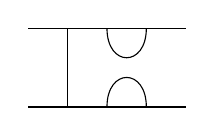
\begin{tikzpicture}
     \draw (0,0) -- (2,0) ;
     \draw (.5,0) -- (.5,-1);
     \draw (1,0) .. controls (1,-.5) and (1.5,-.5) .. (1.5,0) ;
     \draw (1,-1) .. controls (1,-.5) and (1.5,-.5) .. (1.5,-1) ;
 \draw (0,-1) -- (2,-1);
 \end{tikzpicture}
}}
\newcommand{\UI}{
\raisebox{-.32cm}{
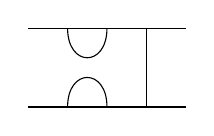
\begin{tikzpicture}
     \draw (0,0) -- (2,0) ;
     \draw (1.5,0) -- (1.5,-1);
     \draw (.5,0) .. controls (.5,-.5) and (1,-.5) .. (1,0) ;
     \draw (.5,-1) .. controls (.5,-.5) and (1,-.5) .. (1,-1) ;
 \draw (0,-1) -- (2,-1);
 \end{tikzpicture}
}}
\newcommand{\SigI}{
\raisebox{-.32cm}{
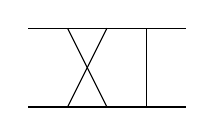
\begin{tikzpicture}
     \draw (0,0) -- (2,0) ;
     \draw (1.5,0) -- (1.5,-1);
     \draw (.5,0) -- (1,-1) ;
     \draw (.5,-1) -- (1,0) ;
 \draw (0,-1) -- (2,-1);
 \end{tikzpicture}
}}

\[ 
\rb{c\;} \begin{tikzpicture}
     \draw (0,0) -- (2,0) ;
     \draw (.5,0) -- (.5,-1);
     \draw (1,0) .. controls (1,-.5) and (1.5,-.5) .. (1.5,0) ;
 \end{tikzpicture}
 \rb{+\;b\;} \begin{tikzpicture}
     \draw (0,0) -- (2,0) ;
     \draw (1,0) -- (1,-1);
     \draw (.5,0) .. controls (.5,-.5) and (1.5,-.5) .. (1.5,0) ;
 \end{tikzpicture}
 \rb{+\;a\;} \begin{tikzpicture}
     \draw (0,0) -- (2,0) ;
     \draw (1.5,0) -- (1.5,-1);
     \draw (.5,0) .. controls (.5,-.5) and (1.0,-.5) .. (1,0) ;
 \end{tikzpicture}
\]
\medskip \medskip 

%\newcommand{\xx}{\alpha}

\noindent 
The action of 
\[
\UI \;\;\;\mbox{ and } \;\;\;  \IU 
\]
must be by 0, so in general 
$\xx a+b+c=0$ and $a+b+\xx c=0$. 
The action of the first elementary transposition
\[
\SigI  
\]
must be by 1 or -1, yielding $b=c$ and $a+2b=0$ in the + case; and $a=0$ and $b=-c$ in the - case, when $\xx=1$. Hence 1d solution spaces. 
(Note that here there is no second elementary transposition! If there were, the system would change radically.)
Thus we see that both one-dimensional $\Delta$-modules are submodules. 
By globalisation this means that we have 
\[
\Delta^{n}_{(3,(2))} \oplus \Delta^{n}_{(3,1^2)} \; \rightarrow\; \Delta^{n}_{(1,(1))}
\]
for all odd $n$, with both summands having nonzero image. 
We draw this as
\[
\hspace{-2.1cm} 
\xymatrix{
   &&&&&& \;\bullet_0 \ar@{-}[d] \\
\ver{(7,\!(2))} \ar@{-}[r] & 
\ver{(6,\!(2))} \ar@{-}[r] & 
\ver{(5,\!(2))} \ar@{-}[r] & 
\ver{(4,\!(2))} \ar@{-}[r]  & 
\ver{(3,\!(2))} \ar@{-}[r] \ar@[red]@/^1.3pc/[rr] & 
\ver{(2,\!(2))} \ar@{-}[r] & 
\bullet_1 \ar@{-}[r] & 
\ver{(2,\!(1^2))} \ar@{-}[r] & 
\ver{(3,\!(1^2))} \ar@{-}[r] \ar@[red]@/_1.3pc/[ll] & 
\ver{(4,\!(1^2))} \ar@{-}[r] & 
\bullet \ar@{-}[r] & 
\bullet \ar@{-}[r] & 
\ver{(7,\!(1^2))} & 
}
\] 

Looking at $n=4$ we see that by Frobenius reciprocity, 
with $A = \Delta^{n-1}_{(3,\lambda)}$ ($\lambda = (2), (1^2)$) and 
$B=\Delta^{n}_{(0,0)}$ in (\ref{eq:FR}), 
we have 
\[
\Delta^{n}_{(4,(2))} \oplus \Delta^{n}_{(4,1^2)} \; \rightarrow\; \Delta^{n}_{(0,(0))}
\]
On the other hand with $A=\Delta^{n-1}_{(3,(2))}$ and $B=\Delta^{n}_{(2,(1^2))}$ we have
\[
\hom(\Delta^{n}_{(4,(2))} \oplus \Delta^{n}_{(2,(2))} , \Delta^{n}_{(2,(1^2))} ) 
 \cong  
\hom(\Delta^{n-1}_{(3,(2))} , \Delta^{n-1}_{(3,(1^2))} + \Delta^{n-1}_{(1,(1))}) 
\]
The sum on the right is non-split, but both factors have $ \Delta^{n-1}_{(3,(2))} $ in the socle, so  the dimension on the right is at least 1. 
And hence also on the left - and by globalisation there is no map from 
$ \Delta^{n}_{(2,(2))}$ to $\Delta^{n}_{(2,(1^2))} $. So we deduce:
\[
\Delta^{n}_{(4,(2))}  \rightarrow   \Delta^{n}_{(2,(1^2))}
\]
(It is worth thinking about other choices for $A$ and $B$!... .) 
And similarly for ... by symmetry. 
Altogether that is:  % \ppm{[unfinished pic!!...]}:
\[
\hspace{-2.1cm} 
\xymatrix{
   &&&&&& \;\bullet_0 \ar@{-}[d] \\
\ver{(7,\!(2))} \ar@{-}[r] & 
\ver{(6,\!(2))} \ar@{-}[r] & 
\ver{(5,\!(2))} \ar@{-}[r] & 
\ver{(4,\!(2))} \ar@{-}[r] \ar@[red]@/^1.3pc/[rrru] \ar@[red]@/^1.9863pc/[rrrr] & 
\ver{(3,\!(2))} \ar@{-}[r] \ar@[red]@/^1.3pc/[rr] & 
\ver{(2,\!(2))} \ar@{-}[r] & 
\bullet_1 \ar@{-}[r] & 
\ver{(2,\!(1^2))} \ar@{-}[r] & 
\ver{(3,\!(1^2))} \ar@{-}[r] \ar@[red]@/_1.3pc/[ll] & 
\ver{(4,\!(1^2))} \ar@{-}[r] \ar@[red]@/_1.3pc/[lllu] \ar@[red]@/_1.93pc/[llll] & 
\bullet \ar@{-}[r] & 
\bullet \ar@{-}[r] & 
\ver{(7,\!(1^2))} & 
}
\] 

Notice that this is consistent with the gram matrix results as in Fig.\ref{fig:Bratelli-l0-gramdets}. 
In particular there is not a morphism from $(4,(2)) \rightarrow (2,(2))$ 
(in the obvious shorthand); nor the symmetry image version. 

Passing on to $n=5$ we see, taking $A=(4,(2))$ and $B=(3,(1^2))$ that 
\[
\hom(\Delta^{n}_{(5,(2))} \oplus \Delta^{n}_{(3,(2))} , \Delta^{n}_{(3,(1^2))} ) 
 \cong  
\hom(\Delta^{n-1}_{(4,(2))} , \Delta^{n-1}_{(2,(1^2))} + \Delta^{n-1}_{(4,(1^2))}) 
\]
Obviously there is a map $(4,(2))\rightarrow (2,(1^2))$, so dim-hom $\geq 1$ on the right unless the $(4,(1^2))$ is glued under - but this would imply a map that we 
noted above  %know 
is not there. Thus dim-hom on the left is nonzero. This forces 
$(5,(2))\rightarrow (3,(1^2))$; and its symmetry image. 
Altogether: 
\[
\hspace{-2.1cm} 
\xymatrix{
   &&&&&& \;\bullet_0 \ar@{-}[d] \\
\ver{(7,\!(2))} \ar@{-}[r] & 
\ver{(6,\!(2))} \ar@{-}[r] & 
\ver{(5,\!(2))} \ar@{-}[r] \ar@[green]@/^2.963pc/[rrrrrr] & 
\ver{(4,\!(2))} \ar@{-}[r] \ar@[red]@/^1.3pc/[rrru] \ar@[red]@/^1.9863pc/[rrrr] & 
\ver{(3,\!(2))} \ar@{-}[r] \ar@[red]@/^1.3pc/[rr] & 
\ver{(2,\!(2))} \ar@{-}[r] & 
\bullet_1 \ar@{-}[r] & 
\ver{(2,\!(1^2))} \ar@{-}[r] & 
\ver{(3,\!(1^2))} \ar@{-}[r] \ar@[red]@/_1.3pc/[ll] & 
\ver{(4,\!(1^2))} \ar@{-}[r] \ar@[red]@/_1.3pc/[lllu] \ar@[red]@/_1.93pc/[llll] & 
\bullet \ar@{-}[r] \ar@[green]@/_3.093pc/[llllll] & 
\bullet \ar@{-}[r] & 
\ver{(7,\!(1^2))} & 
}
\] 
Here there are the possibilities of composite maps:
\[
(5,(2)) \rightarrow (3,(1^2)) \rightarrow (1,(1)) 
\]
and symmetry image. Recall that in the $l=-1$ case all composite maps are zero 
(see \cite[Ch.6]{Martin91}).  
However here we deduce from the gram determinant that 
$ (3,(1^2)) \hookrightarrow (1,(1)) $, and hence the composite is non-zero. 

\subsubsection{Subcase  $(\alpha^2 + \alpha -4)=0$}

\mdef  
Let us have a look at $\alpha$ such that $(\alpha^2 + \alpha -4)=0$. 
Observe from Fig.\ref{fig:Bratelli-l0-gramdets} (say) that 
the first singular gram matrix is for  $\Delta^{4}_{(2,(2))}$. 
By globalisation the only possible maps in are from 
$\Delta^{4}_{(4,(2))}$ or from $\Delta^{4}_{(4,(1^2))}$. 
It is easy to check 
(see e.g. \S\ref{ss:bootcase0})
that there is no  $\Delta^4_{(4,(1^2))}$ subspace
(unless $\alpha=1$), 
so the subspace is $\Delta^4_{(4,(2))}$ here. 
%We can work out which by a little linear algebra. But let us keep going for now. 

By globalisation this means that we have module morphisms 
\beq \label{eq:morphismto22} 
\Delta^n_{(4,(2))}  \rightarrow \Delta^n_{(2,(2))}
\eq 
for all even $n\geq 4$.
%- writing $\lambda \in \{ (2),(1^2) \}$ for the as-yet undetermined partition. 
Thus:
\[
\hspace{-2.1cm} 
\xymatrix{
   &&&&&& \;\bullet_0 \ar@{-}[d] \\
\ver{(7,\!(2))} \ar@{-}[r] & 
\ver{(6,\!(2))} \ar@{-}[r] & 
\ver{(5,\!(2))} \ar@{-}[r] & 
\ver{(4,\!(2))} \ar@{-}[r] \ar@[red]@/^1.3pc/[rr] & 
\ver{(3,\!(2))} \ar@{-}[r] & 
\ver{(2,\!(2))} \ar@{-}[r] & 
\bullet_1 \ar@{-}[r] & 
\ver{(2,\!(1^2))} \ar@{-}[r] & 
\ver{(3,\!(1^2))} \ar@{-}[r] & 
\ver{(4,\!(1^2))} \ar@{-}[r] & 
\bullet \ar@{-}[r] & 
\bullet \ar@{-}[r] & 
\ver{(7,\!(1^2))} & 
}
\]

The next singularity is for $\Delta^{5}_{(1,(1))}$. 
The map in here is from 
$\Delta^{5}_{(5,(2))}$ or from $\Delta^{5}_{(5,(1^2))}$. 
By Frobenius reciprocity 
- see (\ref{exa:henri1}) below for details - 
the $\lambda\in\{ (2),(1^2)\}$ will be the same as for the first map above. 
Thus we have 
\beq \label{eq:morphismto11} 
\Delta^n_{(5,\lambda)}  \rightarrow \Delta^n_{(1,(1))}
\eq 
with $\lambda=(2)$, 
for all odd $n \geq 5$. 
%Let us continue. 
Thus: 
\[
\hspace{-2.1cm} 
\xymatrix{
   &&&&&& \;\bullet_0 \ar@{-}[d] \\
\ver{(7,\!(2))} \ar@{-}[r] & 
\ver{(6,\!(2))} \ar@{-}[r] & 
\ver{(5,\!(2))} \ar@{-}[r]  \ar@[red]@/^1.7pc/[rrrr] & 
\ver{(4,\!(2))} \ar@{-}[r] \ar@[red]@/^1.3pc/[rr] & 
\ver{(3,\!(2))} \ar@{-}[r] & 
\ver{(2,\!(2))} \ar@{-}[r] & 
\bullet_1 \ar@{-}[r] & 
\ver{(2,\!(1^2))} \ar@{-}[r] & 
\ver{(3,\!(1^2))} \ar@{-}[r] & 
\ver{(4,\!(1^2))} \ar@{-}[r] & 
\bullet \ar@{-}[r] & 
\bullet \ar@{-}[r] & 
\ver{(7,\!(1^2))} & 
}
\]

At $n=6$ we already have a map from  (\ref{eq:morphismto22}). 
Note that this explains the $(\alpha^2+\alpha-4)^6$ in the gram-det of 
$ \Delta^6_{(2,(2))}  $, since the map is   %both possible maps are 
from a 6-dimensional simple module. 
In addition we have two further singularities here, for 
$ \Delta^6_{(0,(0))}  $    and   $ \Delta^6_{(2,(1^2))}  $. 
By Frobenius reciprocity it seems that both should be from 
$ \Delta^6_{(6,\lambda=(2))}  $. %\ppm{[-but this should be checked!]}\bajm{(has been!)}. 
Altogether we add to the figure as shown in red in Fig.\ref{fig:standardmapshenri}. 
%\ppm{[oh dear, something has gone wrong with colours!! - fixed by adding [all] to xypic, but odd because it was working before.]}

\begin{figure}
\[
\hspace{-2.1cm} 
\xymatrix{
   &&&&&& \;\bullet_0 \ar@{-}[d] \\
\ver{(7,\!(2))} \ar@{-}[r] \ar@[green]@/^2.643pc/[rrrrrr] \ar@[green]@/^3.643pc/[rrrrrrrr] & 
\ver{(6,\!(2))} \ar@{-}[r] \ar@[red]@/^1.7pc/[rrrrru] \ar@[red]@/^2.1pc/[rrrrrr] & 
\ver{(5,\!(2))} \ar@{-}[r]  \ar@[red]@/^1.7pc/[rrrr] & 
\ver{(4,\!(2))} \ar@{-}[r] \ar@[red]@/^1.3pc/[rr] & 
\ver{(3,\!(2))} \ar@{-}[r] & 
\ver{(2,\!(2))} \ar@{-}[r] & 
\bullet_1 \ar@{-}[r] & 
\ver{(2,\!(1^2))} \ar@{-}[r] & 
\ver{(3,\!(1^2))} \ar@{-}[r] & 
\ver{(4,\!(1^2))} \ar@{-}[r] & 
\bullet \ar@{-}[r] & 
\bullet \ar@{-}[r] & 
\ver{(7,\!(1^2))} & 
}
\]
    \caption{ Standard module morphisms for $l=0$ for $(\alpha^2+\alpha-4)=0$. \label{fig:standardmapshenri} }
\end{figure}


At $n=7$ we already have a map from (\ref{eq:morphismto11}). 
Note that this explains a factor $(\alpha^2+\alpha-4)^7$ in the gram-det of $\Delta^7_{(1,(1))}$. 
But in fact the exponent is 8. 
On the other hand we can consider if Frobenius reciprocity gives us a map in 
also from $ \Delta^7_{(7,\lambda)}$.  
%\ppm{[paul, do this calculation!]}
In that case we would have two socle factors. 
The other singular case is $(3,(1^2))$, but for this just consider Frobenius reciprocity applied to 
$   \Delta^6_{(6,\lambda)} \rightarrow   \Delta^6_{(2,(1^2))}  $ 
from above. 
See the red and green arrows in Fig.\ref{fig:standardmapshenri}. 

\mdef  \label{pa:FR}   {\bf{Frobenius reciprocity}}. 
Here we briefly review and apply the {\em tower of recollement} method of \cite{ToR}. 
Recall that given an inclusion of algebras $ X \subset Y$ and an $X$-module $A$ and
a $Y$-module $B$, 
then Frobenius reciprocity is the isomorphism of hom-spaces
\beq \label{eq:FR} 
\hom_Y(Ind\;A,B) \cong \hom_X(A,Res\;B)
\eq 
where $Ind-$ and $Res-$ refer to the induction and restriction along $ X \subset Y$. 

\mdef   \label{exa:henri1}
For example consider $J_{0,n-1} \subset J_{0,n}$ with $(\alpha^2+\alpha-4)=0$. 
From (\ref{eq:morphismto22}) above we have the map  
$ \Delta^n_{(4,(2))}  \rightarrow \Delta^n_{(2,(2))} $ ($n$ even). 
Now note that when $n=5$ we have 
\[
Res \; \Delta^n_{(1,(1))} =  \Delta^{n-1}_{(2,(2))} \oplus \Delta^{n-1}_{(2,(1^2))} \oplus \Delta^{n-1}_{(0,(0))}
\]
(it is a general result for all $n$ odd that the factors on the right are filtration factors, but here they are in different blocks)
so we see that 
$$
\hom(\Delta^{n-1}_{(4,(2))}, Res \; \Delta^n_{(1,(1))}) \neq 0   .
$$ 
By reciprocity therefore 
$$
\hom_Y(Ind\; \Delta^{n-1}_{(4,(2))},  \Delta^{n}_{(1,(1))}) \neq 0   .
$$ 
We have 
\[
Ind\; \Delta^{n-1}_{(4,(2))} = \Delta^n_{(5,(2))} \oplus \Delta^n_{(3,(2))}
\]
- certainly a direct sum when $n=5$. There is no map 
$ \Delta^n_{(3,(2))} \rightarrow \Delta^n_{(1,(1))} $ 
- else it would have an image at lower $n$ by localisation. 
Thus we must have a map $ \Delta^n_{(5,(2))} \rightarrow \Delta^n_{(1,(1))} $. 

\medskip 

The above example  confirms completely what we already part-deduced from the gram-dets in our argument for $n=5$. 
Now let us try the same method for the $n=6$ cases. 
Consider
\[Res(\Delta^6_{(0,(0))})= \Delta^5_{(1,(1))}  \qquad  Res(\Delta^6_{(2,(1^2))})= \Delta^5_{(1,(1))}\oplus \Delta^5_{(3,(1^2))}\]
Therefore, we have 
\[  \hom(\Delta^5_{(5,(2))}, Res\Delta^6_{(0,(0))})\neq 0\]
hence
\[\hom(Ind\Delta^5_{(5,(2))}, \Delta^6_{(0,(0))})\neq 0\]
and $Ind\Delta^5_{(5,(2))}=\Delta^6_{(4,(2))} \oplus \Delta^6_{(6,(2))}$, we would have seen maps $\Delta^6_{(4,(2))}\to \Delta^6_{(0,(0))}$ at a lower stage so we must have $\Delta^6_{(6,(2))}\to \Delta^6_{(0,(0))}$ (and likewise $\Delta^6_{(6,(2))}\to \Delta^6_{(2,(1^2))}$ ).
%\ppm{[-almost finished!]}




